% !TEX root = main.tex

\section{Lecture 9: Numerics: Horizontal Discretisation}
% please write the title when you start writing the notes
% this way I know by glancing the table of contents where to look
% cheers, Navid
\begin{flushright}\textbf{[by Stefan Jendersie]}\end{flushright}

\begin{figure}
\begin{center}
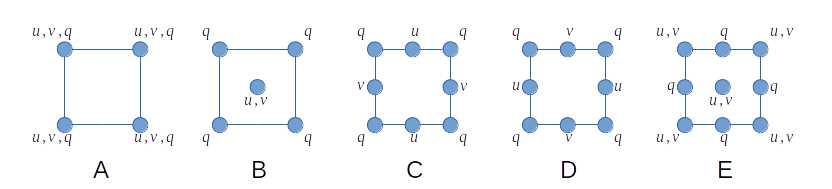
\includegraphics[scale=0.7]{lecture09_arakawa_grids.png}
\label{fig:arakawa_grid}
\caption{Numerical arrangement of ocean dynamical and state variables in \textit{Arakawa grids}. $u$ and $v$ are velocities, $q$ stands for properties of state such as density, temperature, biological tracers concentrations etc. }
\end{center}
\end{figure}
%
In order to numerically solve the equation of motion and the tracer advection in an ocean model the 3-D geophysical domain can be subdivided into a discrete set of grid points (finite difference).  Each physical variable defined at the grid point location represents a mean over the volume associated with the grid point. Conveniently the discretised domain is mapped onto a computationally meaningful structure by use of a logic 3-D array.  While the vertical mapping is established in Section \ref{sec:???} we here introduce the mapping of the horizontal discretisation.
%
\paragraph*{}
The $x$ component of the in-compressible Navier-Stokes equation as derived in Section \ref{???}(p32) where we omit the diffusion and stress terms writes as
\begin{equation}
  \frac{\partial uh}{\partial t} + \frac{\partial uuh}{\partial x} + \frac{\partial vuh}{\partial y} - fhv = g' h \frac{\partial \eta_1}{\partial x} + ...
\end{equation}
Assume a constant depth $h=H$ with $\eta_1\approx h$ and zero velocities with a non vanishing time derivative
\begin{equation}
     u=0+u' \qquad v=0+v'
\end{equation}
gives
\begin{equation}
\frac{\partial u}{\partial t}  = g'\frac{\partial h}{\partial x} + fv. \label{eqn:uEOM}
\end{equation}

%
As shown in Section \ref{???} (p31) integrating the expression for an incompressible fluid 
\begin{equation}
 \boldsymbol{\nabla}\cdot\boldsymbol{v} = 0
\end{equation}
over the water depth $h$ yields 
\begin{equation}
\frac{\partial h}{\partial t} + \frac{\partial (uh)}{\partial x} + \frac{\partial (vh)}{\partial y} = 0.\label{eqn:boussinesq}
\end{equation}
By splitting the depth into a constant and a time dependent term $h = H+h'(t)$ this becomes 
\begin{equation}
\frac{\partial h}{\partial t} + H\left(\frac{\partial u}{\partial x} + \frac{\partial v}{\partial y}\right) = 0.
\end{equation}
%
%
Let $\tau$ and $i$ be the time level and the horizontal index in $x$ direction.  Writing out in its discrete form and centred on the current time step $\tau$: the $u$ component in Eqn \ref{eqn:uEOM} 
%
\begin{equation}
\frac{u_i^{\tau+1} - u_i^{\tau-1}}{2\Delta t} = \frac{g'(h^\tau_{i+1}-h^\tau_{i-1})}{2\Delta x} + fv_{i}^{\tau}
\end{equation}
\begin{equation}
u_i^{\tau+1} - u_i^{\tau-1} =  \frac{g'\Delta t}{\Delta x} (h^\tau_{i+1}-h^\tau_{i-1}) + 2\Delta t fv_{i}^{\tau}
\end{equation}
and the Boussinesq Approximation in Eqn \ref{eqn:boussinesq}
\begin{eqnarray}
h_i^{\tau+1}-h_i^{\tau-1} = \frac{-H \Delta t}{\Delta x} (U^\tau_{i+1}-U^\tau_{i-1})
\end{eqnarray}
%
give expressions for the logical (and geophysical) spatial and temporal relationship of the involved  variables, e.g. the equations' footprint.  The nature of how partial derivatives are discretised in their simplest form relates position $i$ of $u$ at times $\tau-1$ and $\tau+1$ to $i+1$ and $i-1$ of $h$ at 
$\tau$ and vice versa.  
\paragraph*{}
If $h$ and $u$ are simply defined at the same horizontal locations $i$, i.e. arranged as an unstaggered \textit{Arakawa A-Grid} (Figure \ref{fig:arakawa_grid}), this would create two tempo-spatially entangled but physically decoupled grids, e.g. much like a checkerboard where white and black fields only communicate with fields alike (Figure \ref{fig:decoupled_grid}). 
%

\begin{figure}
\begin{center}
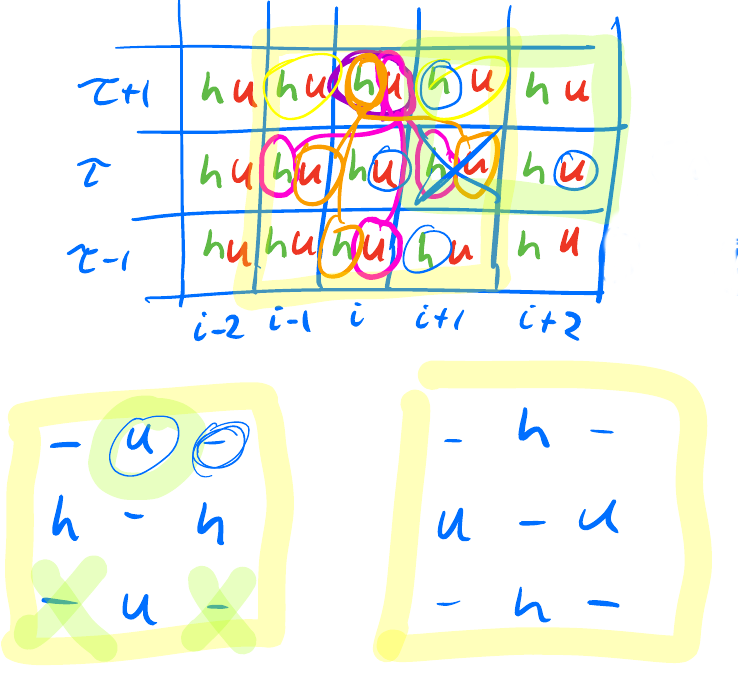
\includegraphics[scale=0.5]{lecture09_Agrid_footprint}
\label{fig:decoupled_grid}
\caption{Footprint of Equation \ref{eqn:uEOM} on an \textit{Arakawa A-grid}. Two entangled but independent grids resulting from velocity and depth being defined in the same location (from handwritten AOMSS lecture notes).}
\end{center}
\end{figure}
%
\paragraph*{}
By no means dismissing the A-grid's usefulness for other computational problems in the case outlined here arranging variables in a staggered grid is more efficient.
Arakawa grids offer different types of staggering.  If the problem was solved on a B-grid (Figure \ref{fig:arakawa_grid}) the partial derivative of $h$ (Eqn. \ref{eqn:part_der}) centres between velocity points in $j$ direction (red crosses in Figure \ref{fig:B_Cgrid}), hence requiring another computation to average the derivative onto the velocity position (Eqn \ref{eqn:avg_j};  blue $u$/$v$ arrows in Figure \ref{fig:B_Cgrid}):  
%
\begin{align}
\rightarrow \delta_x &= \left[(\quad )_{i+\frac{1}{2}} - (\quad )_{i-\frac{1}{2}}  \right] \frac{1}{\Delta x}  \nonumber \\
\delta_x h &= \left[(h)_{i+\frac{1}{2}} - (h)_{i-\frac{1}{2}}  \right] \frac{1}{\Delta x} \label{eqn:part_der}\\
\rightarrow \overline{(\quad)}^y &= \left[ (\quad )_{j+\frac{1}{2}} + (\quad )_{j-\frac{1}{2}}  \right] \frac{1}{2}  \nonumber \\
(\delta_x h)_{i,j} &= \left[ (\delta_x h)_{j+\frac{1}{2}} + (\delta_x h)_{j-\frac{1}{2}}  \right] \frac{1}{2}. \label{eqn:avg_j}
\end{align} 
%
%
\begin{figure}
\begin{center}
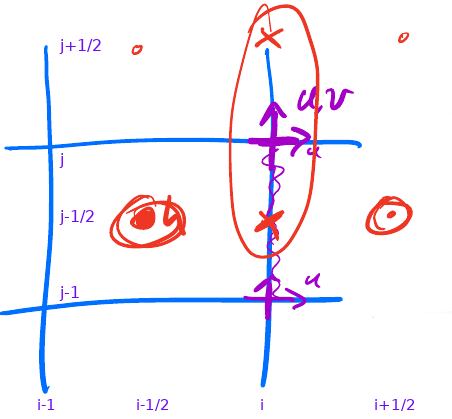
\includegraphics[scale=0.5]{lecture09_B_grid_02}
\label{fig:B_Cgrid}
\caption{Footprint of Equation \ref{eqn:uEOM} on an \textit{Arakawa B-grid} (modified from handwritten AOMSS lecture notes, added grid indices).}
\end{center}
\end{figure}
%
Using expressions \ref{eqn:part_der} and \ref{eqn:avg_j} Equation \ref{eqn:uEOM} on a B-grid becomes
\begin{align}
\frac{\partial u_{ij}}{\partial t} &= fv_{ij} + g'\overline{\frac{h_{i+\frac{1}{2}} - h_{i-\frac{1}{2}}}{\Delta x_i}}^y \\
&= fv_{ij} + \frac{g'}{2}\left( 
\frac{h_{i+\frac{1}{2},j-\frac{1}{2}} - h_{i-\frac{1}{2},j-\frac{1}{2}}}{\Delta x_{i,j-\frac{1}{2}}} + 
\frac{h_{i+\frac{1}{2},j+\frac{1}{2}} - h_{i-\frac{1}{2},j+\frac{1}{2}}}{\Delta x_{i,j+\frac{1}{2}}} \right) \\
&= fv_{ij} + g' \delta_xh_{ij}.
\end{align}
The equation's footprint for $h$ is 4 and requires three sum and two division operations (or multiplication by the inverse of $\Delta x$).  While in an \textit{Arakawa C-Grid} (Figure \ref{fig:arakawa_grid}) the footprint of $h$ reduces to 2, one sum and one division, $v$ now requires an averaging operation over a footprint of 4 as the velocity field itself is arranged in a staggered form 
\begin{equation}
\frac{\partial u_{ij}}{\partial t} = f \overline{\overline{v_{ij}}^x}^y + g'\delta_x h.
\end{equation}
It becomes clear that the choice of arranging the physical variables in an ocean model should ideally suit the problem to be solved.  For example in solutions where the curl of the velocity field is frequently needed a \textit{B-grid} or an \textit{E-grid} might be more suitable as both velocity components are readily defined in the same location.
%
%For example in a Arakawa C or E grid arrangement the differences (discretized partial derivatives) of the dynamical variables are naturally centred on the position of the state variables. 

